\documentclass[a4paper,12pt]{article}
\usepackage[utf8]{inputenc}
\usepackage[T1]{fontenc}
\usepackage[british]{babel}
\usepackage{hyperref}
%\usepackage[margin=1in]{geometry}
\usepackage{listings}
\usepackage{xspace}
\usepackage{graphicx}
\usepackage{indentfirst}

\title{Gomat specification}
\author{Gauthier Jolly \and K\'{e}vin Car\'{e}nou \and Matei Oltean}

\newcommand{\Gossiper}{\texttt{Gossiper}\xspace}
\newcommand{\Gomat}{\texttt{Gomat}\xspace}
\newcommand{\Go}{\texttt{Go}\xspace}

\begin{document}
\maketitle
\tableofcontents
\newpage
    \section{Introduction}
    \Gomat is a tool which allows users to compute complex operation on matrices on a computer network.
    \Gomat is in the same time a \texttt{Go API} and a daemon. By running the daemon, a user becomes part of a network and can use the \texttt{Go API} to execute big computations.

    \section{Goal and Functionalities}
        \subsection{Daemon}
    When a user wants to join a \Gomat network, it has to run the dedicated daemon. The daemon is the main component of the application. It splits and merges, executes computations and communicates with other peers. For this last point, it uses a \Gossiper network.

        \subsubsection{GUI}
    On the \texttt{GUI}, the client can change the maximum number of computations his computer can do at a time. He can see the number of computation his computer has done, check the peers he knows, see the ratio $r =$ number of computation tasks sent/{number of computation tasks computed}.

        \subsection{API}
        Our API is a \Go package which is used to communicate with the daemon. When a user wants to compute an operation between to big matrices, he calls\\
    \texttt{Gomat.compute(matrix1, matrix2 Matrix, operation Gomat.Operation) (result Matrix, err error)}

        \subsection{Failure management}
    Since it is a decentralised system where one peer delegates part of its job to others, it is essential to detect failures, manage them, and implement methods that make the system more resilient.

    It must be noted that failure detection and management work both ways. For a given computation, the gossiper that wants its job done must detect failing peers, so that it does not have to wait forever for their reply---and it should sent the dropped task to other peers for computations---, but ‘computing’ gossiper want to detect if the node that send them tasks fails, so that they can drop the job and reallocate their resources.

    \section{Design and Architecture}
    \begin{figure}[!ht]
        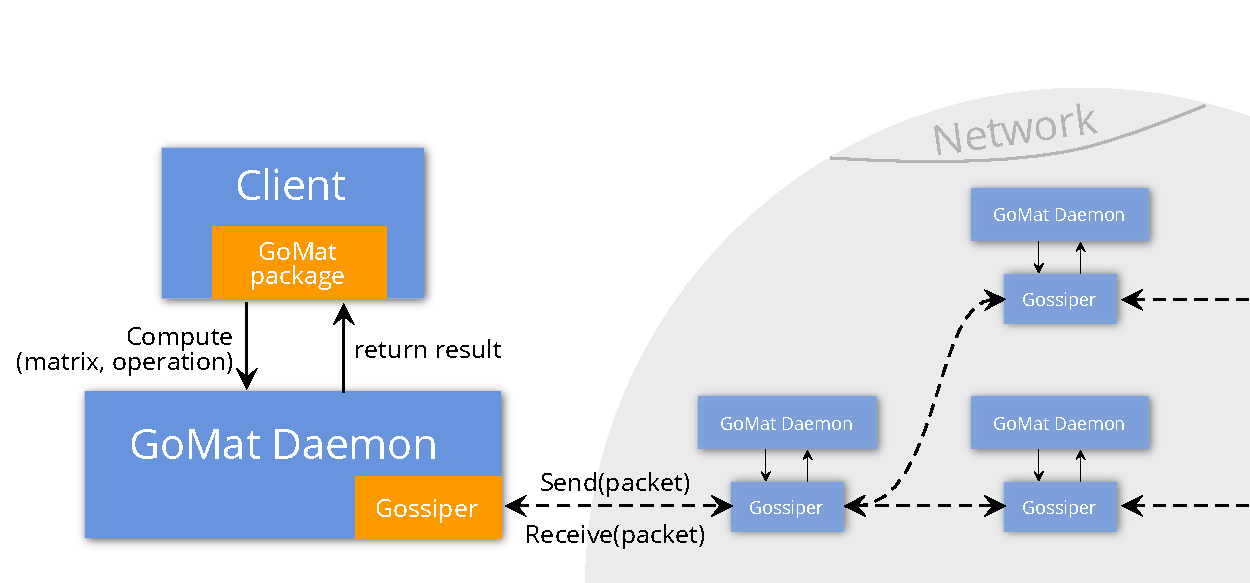
\includegraphics[width=.95\textwidth]{global_view.pdf}
        \caption{Global view}
        \label{glbView}
    \end{figure}
    \begin{figure}[!ht]
        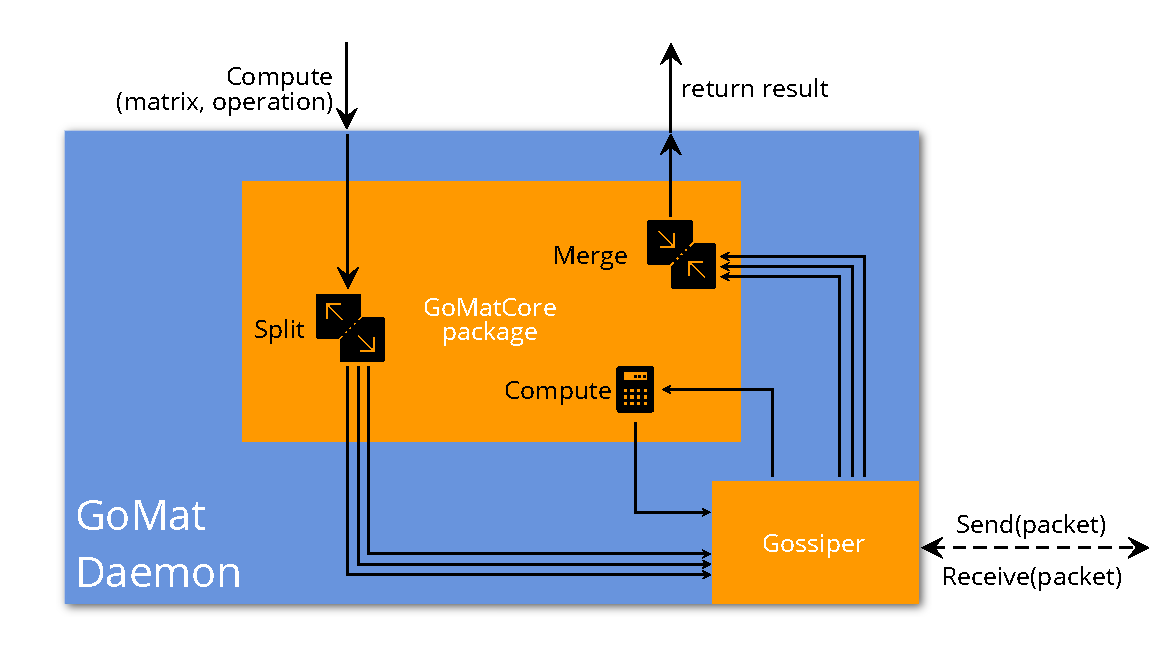
\includegraphics[width=.95\textwidth]{daemon_view.pdf}
        \caption{Daemon architecture}
        \label{daemonView}
    \end{figure}
        \subsection{Daemon}
        The creation of GoMatCore package and the demonstration application will be supervised by Kévin Carenou.

        A \Gomat peer is not a \Gossiper peer, but contains a \Gossiper peer that it uses to send and receive messages. Our \Gomat application uses the \Gossiper as a transport layer (layer 4).

        \subsubsection{GUI}
        Once the daemon is running, it is not automatically connected to a \Gomat network. The user has to open a web browser and go on \url{http://localhost:8080} (can be modified in a configuration file) to add some peers to be connected on a
    \Gomat network.

    \subsubsection{Split, merge and computation}
    When receiving a computation request from the API, the daemon will split the input matrices into smaller submatrices, to be sent to the network for computations.

    When a peer's deamon accept to compute a chunk of data, this deamon will do the computation using the \texttt{GoMatCore} package. This package implements functions computing the different operations.

    After receiving the results of the computations, the daemon merges the subresults into a result matrix.

    \subsection{API}
    The API in charge of the communication between the application and the Daemon will be implemented by Gauthier Jolly.

    Our API is a \Go package which is used to communicate with the daemon. When an application wants to compute an operation between to big matrices, he calls:\\
    \texttt{Gomat.compute(matrix1, matrix2 Matrix, operation Gomat.Operation) (result Matrix, err error)}


    This function is blocking.

    If there is no \Gomat daemon running on the computer, \texttt{Gomat.compute} returns an error.

        \subsubsection{Communications between API and Daemon}
    The application using the API and the Daemon are running on the same computer. Thus, there is no need to use the network (i.e. the loopback interface).
    We use \texttt{Inter-Process Communication (IPC) sockets} to send information between the daemon and the API.

        \subsection{Failure management}
        Failure detection will be supervised by Matei Oltean.

        \subsubsection{Detecting failures}
    To manage failures, we first need to detect them.

    When \texttt{Gomat.compute} is used, the \Gomat daemon will first check that all of its peers are working. To that effect, it will send them a particular message and will wait for an acknowledgement. If after some time, some do not reply, they will be considered to have failed, will be removed from the list of peers, and no task will be sent to them.

~~

    Whenever a ‘master’ gossiper splits a computation and sends it to peers for computing, it creates a routine for each contacted gossiper, that listens and writes to it.
When a gossiper receives the job, it acknowledges it by sending an answer to the master gossiper.
Then, the master will send back a message to the gossiper, who will reply, and so one.

    If at any point, a gossiper times out when listening (i.e. it does not receive an answer fast enough), the other node is considered to have failed.

~~

    It must be noted that such a message coming from an unknown peer is received, it will be added to the list of potential peers.

    \subsubsection{Failure management}
    When a gossiper $g$ finds that another one, $a$, has failed, it will be removed from the list of peers, the routine created to communicate with $a$ will be killed and one of the three will occur:

\begin{itemize}
\item If $a$ was doing some computation for $g$, $g$ will split the computation between its remaining peers.
\item If $g$ was doing some computation for $a$, $a$ will stop its computation.
\item In any other case, nothing more will be done.
\end{itemize}

    \subsubsection{Making the system more resilient}
    If a gossiper $g$ receives a task and has enough idle peers, it can redistribute some of it amongst them. There must be some wait time (maybe they have all received subtasks from the same job, but because of delays, $g$ still sees them as idle).
In that case, the ‘master’ peer must be informed of their computations, they will be added to its peers, and as for others, it must now detect their failures.

    Then, if $g$ crashes, not all of the computations sent to him will have to be redone, since some subtasks are now processed by its peers.

    The master node will also be able to add gossipers to its list of known peers, and the network will be more robust.

    \section{Evaluation Plan}
    First, we need to be sure, that the matrix splitting, merging, and the operations on them behave as they should.

    When implementing them, we have proved that, mathematically, they should work. But we must still test them, and we will do that both locally, and, once it works, with a small network.
    
    [TODO TESTS UNITAIRES]
    
    Since most of the tests will be run through the API, we must also check that when \texttt{Gomat.compute} is executed, the correct tasks are run in the background.

~~
    
    Since the message spreading is built on top of Peerster, it should work and is already tested. Obviously, the messages sent for computations and failure detection are different from GossipPackets, but we will check if everything works when testing our parts of the program.
    
~~
    
    For the failure detection, we will have to check two things (and also adapt the timeout parameters accordingly): that if a peer fails, the other detect it fast, and that there a very few false positives (i.e. that a node is seen as having failed, while it still runs fine). We will simulate small networks, with failing nodes (i.e. deconnexions), and check the reactions of the remaining gossipers.
    
    We will also check that when a node receives a message, it always adds the sender to its list of known peers, by sending blank messages (we must also be sure that a message not well formatted is discarded, instead of making the node thread crash).
    
~~

    While all those tests will be running, we will have a GUI running, and we will check that all the informations displayed are correct.

    \section{Conclusion}
    These specifications are meant to change, since it is only a second draft.

    For example, a function of preference should be added. The sizes of the matrices sent for computations should depend on the computation power of the gossiper, its response time,~etc. But for that, we would also need to optimise the splitting and merging parts, in order to be able to efficiently merge submatrices of different sizes.
\end{document}
